\section{Experiments}\label{sec:exp_setup}
% We evaluate our algorithms on real-word datasets that are extensive and representative for federated learning. The objective is to gain a deeper understanding of the impact of period drift and client drift, and the interaction on the convergence of cross-device FL. To accomplish this, we conduct simulations on four datasets. Each of the datasets includes at least three non-iid settings, established through the Dirichlet distribution partition method\citep{hsu2019measuring}, and one of them has a naturally-arising client partitioning setting in real-world FL scenarios, thereby making it highly representative.
\begin{table}[t]
    \centering
    \caption{\small\textbf{Results on FEMNIST and CIFAR-100.} The best method is highlighted in \textbf{bold} fonts.}
    \resizebox{0.9\linewidth}{!}{ % Adjusted width for single column table
    \begin{tabular}{l|cccc|ccc}
    \toprule
    Dataset&\multicolumn{4}{c}{FEMNIST}&\multicolumn{3}{c}{CIFAR-100}\\
    \cmidrule(lr){1-5}
    \cmidrule(lr){6-8}
    Methods/NonIID &natural &$\alpha=1$ &$\alpha=0.1$ &$\alpha=0.01$&$\alpha=1$ &$\alpha=0.1$ &$\alpha=0.01$\\
    \midrule
    \fedavg & 82.37 $\pm$ 0.18 & 83.60 $\pm$ 0.11 & 82.02 $\pm$ 0.23 & 73.23 $\pm$ 1.36 &47.04 $\pm$ 0.21 &43.93 $\pm$ 0.36 & 30.11 $\pm$ 0.53 \\
    \fedavgm & 82.53 $\pm$ 0.43 & 83.67 $\pm$ 0.10 & 82.30 $\pm$ 0.49 & 74.96 $\pm$ 2.34 & 48.22 $\pm$ 0.19 & 44.74 $\pm$ 0.40 &31.59 $\pm$ 0.98 \\
    \fedprox & 82.34 $\pm$ 0.17 & 83.58 $\pm$ 0.11 & 82.04 $\pm$ 0.27 & 74.16 $\pm$ 1.19 &46.86 $\pm$ 0.38 &43.74 $\pm$ 0.27 &30.10 $\pm$ 0.55 \\
    \scaffold & 81.66 $\pm$ 0.28 & 83.06 $\pm$ 0.14 & 79.82 $\pm$ 0.42 & 5.13 $\pm$ 0.00 &47.26 $\pm$ 1.49 &36.36 $\pm$ 4.98 &1.00 $\pm$ 0.00 \\
    \fedopt & 5.13 $\pm$ 0.00 & 81.86 $\pm$ 0.38 & 78.13 $\pm$ 0.39 & 5.13 $\pm$ 0.00 &47.26 $\pm$ 1.49 &45.43 $\pm$ 1.18&32.17 $\pm$ 1.38 \\
    \rowcolor{Gray}
    \textbf{\fedeve}&\textbf{82.68 $\pm$ 0.19} &\textbf{83.81 $\pm$ 0.09} &\textbf{82.69 $\pm$ 0.31} &\textbf{75.99 $\pm$ 1.61} &\textbf{48.38 $\pm$ 0.24} &\textbf{45.68 $\pm$ 0.16} &\textbf{32.68 $\pm$ 0.62} \\
    \bottomrule
    \end{tabular}
    }
    \label{tab:femnist_cifar100}
\end{table}

\begin{table}[t]
    \centering
    \caption{\small\textbf{Results on MovieLens-1M.} The best method is highlighted in \textbf{bold} fonts.}
    \resizebox{0.9\linewidth}{!}{% Adjusted width for single column table
    \begin{tabular}{@{}lcccccc@{}}
    \toprule
    & AUC & HR@5 & HR@10 & NGCG@5 & NGCG@10 \\
    \midrule
    \fedavg & 0.7633 $\pm$ 0.0065 & 0.2774 $\pm$ 0.0100 & 0.4294 $\pm$ 0.0120 & 0.1835 $\pm$ 0.0058 & 0.2324 $\pm$ 0.0064 \\
    \fedavgm & 0.7555 $\pm$ 0.0128 & 0.2705 $\pm$ 0.0384 & 0.4290 $\pm$ 0.0196 & 0.1771 $\pm$ 0.0319 & 0.2280 $\pm$ 0.0257 \\
    \fedprox & 0.7819 $\pm$ 0.0033 & 0.2700 $\pm$ 0.0129 & 0.4279 $\pm$ 0.0083 & 0.1803 $\pm$ 0.0078 & 0.2310 $\pm$ 0.0065 \\
    \fedopt & 0.7751 $\pm$ 0.0085 & 0.2868 $\pm$ 0.0055 & 0.4392 $\pm$ 0.0101 & 0.1886 $\pm$ 0.0044 & 0.2377 $\pm$ 0.0040 \\
    \rowcolor{Gray}
    \fedeve & \textbf{0.7967 $\pm$ 0.0016} & \textbf{0.2916 $\pm$ 0.0077} & \textbf{0.4460 $\pm$ 0.0088} & \textbf{0.1924 $\pm$ 0.0039} & \textbf{0.2407 $\pm$ 0.0037} \\
    \bottomrule
    \end{tabular}
    }
    \label{tab:ml-1m}
\end{table}

\subsection{Setup}
\textbf{Datasets and models.} We evaluate \fedeve on three computer vision (CV) and recommender system (RS) datasets under realistic cross-device FL settings. \emph{\textbf{For CV dataset}}, we use FEMNIST\footnote{https://github.com/TalwalkarLab/leaf/tree/master/data/femnist} \cite{caldas2018leaf}, consisting of 671,585 training examples and 77,483 test samples of 62 different classes including 10 digits, 26 lowercase and 26 uppercase images with 28x28 pixels, handwritten by 3400 users. 
We also use CIFAR-10/100 \footnote{https://www.cs.toronto.edu/~kriz/cifar.html} \cite{caldas2018leaf}, consisting of 50,000 training examples and 10,000 test samples of 10/100 different classes with 32x32 pixels. For FEMNIST dataset, we use the lightweight model LeNet5 \cite{lecun1998gradient} and for CIFAR-10/100 dataset, we use ResNet-18 (replacing batch norm with group norm \citep{hsieh2020non,reddi2020adaptive}).
\emph{\textbf{For RS dataset}}, we use MovieLens 1M \footnote{https://grouplens.org/datasets/movielens/}\cite{harper2015movielens}, including 1,000,209 ratings by unidentifiable 6,040 users on 3,706 movies. It is a click-through rate (CTR) task, and we use the popular DIN \cite{zhou2018deep} model. For performance evaluation, we follow a widely used leave-one-out protocol \cite{muhammad2020fedfast}. For each user, we hold out their latest interaction as testset and use the remaining data as trainset, and binarize the user feedback where all ratings are converted to 1, and negative instances are sampled 4:1 for training and 99:1 for test times the number of positive ones.



\textbf{Federated learning settings.}
It is important to note that the datasets FEMNIST and MovieLens 1M have a "natural" non-iid distribution, which means that the data is split by ``user\_id''. For example, in FEMNIST, images are handwritten by different users, and in MovieLens 1M, movies are rated by different users. Furthermore, we use the Dirichlet distribution, to simulate the label distribution skew setting for FEMNIST, as described in \cite{hsu2019measuring}. This distribution allows us to control the degree of heterogeneity by adjusting the hyperparameter $\alpha$ (the smaller, the more non-iid). This allows us to test the robustness of the algorithm under different levels of heterogeneity, which is a common scenario in real-world FL settings. For the FL training, we set a total of $T=1500$ communication rounds for the CV task and sample $10$ clients per round with SGD optimizer. For the RS task, we set a total of $T=1000$ communication rounds and sample $20$ clients per round with Adam optimizer \cite{kingma2014adam}. In all datasets, each client trains for $E=1$ epoch at the local update with a learning rate of $\eta_l=0.01$. In our proposed \fedeve, we set the global learning rate $\eta_g=1$ for all experiments.

\textbf{Baselines.}
To evaluate the performance of \fedeve, we compare it with several state-of-the-art FL methods: 1) The vanilla FL method \fedavg \cite{mcmahan2017communication}, which is a widely used method for FL; 2) A client-side FL method \fedprox \cite{li2020federated}, which improves the model aggregation by adding a proximal term to the local update; 3) A server-side FL method \fedavgm \cite{hsu2019measuring}, which adapts the momentum in FL optimization; 4) A server-side FL method \fedopt \cite{reddi2020adaptive}, which introduces adaptive optimization methods in FL. See more experimental details in the Appendix \ref{exp:metrics}. \looseness=-1



% to appendix
% \textbf{Evaluation Metrics.}
% In our experiments, the performance of the model for the CV tasks is evaluated using the widely accepted metric of Top-1 accuracy. For the RS task, several popular metrics are used to measure the performance of the model, such as the area under the curve (AUC), Hit Ratio (HR), and Normalized Discounted Cumulative Gain (NDCG). These metrics are commonly used in RS to evaluate the performance for click-through rate prediction tasks:
% \begin{equation*}
%   \small
%   \begin{aligned}
%   &\mathrm{AUC}=\frac{\sum_{x_{0} \in D_{T}} \sum_{x_{1} \in D_{F}} \mathbf{1}\left[f\left(x_{1}\right)<f\left(x_{0}\right)\right]}{\left|D_{T}\right|\left|D_{F}\right|},\\
%   &\text { HitRate@K }=\frac{1}{|\mathcal{U}|} \sum_{u \in \mathcal{U}} \mathbf{1}\left(R_{u, g_{u}} \leq K\right), \\
%   &\text { NDCG@K }=\sum_{u \in \mathcal{U}} \frac{1}{|\mathcal{U}|} \frac{2^{\mathbf{1}\left(R_{u, g_{u}} \leq K\right)}-1}{\log _{2}\left(\mathbf{1}\left(R_{u, g_{u}} \leq K\right)+1\right)},
%   \end{aligned}
% \end{equation*}
% where $\mathcal{U}$ represents the set of users, $\mathbf{1}$ is the indicator function, $R_{u, g_{u}}$ represents the rank generated by the model for the ground truth item $g_{u}$, $f$ represents the model being evaluated, $D_{T}$ represents the positive sample set, and $D_{F}$ represents the negative sample set in the testing data. 
  
% put it in appendix: To provide a clearer illustration, we displayed the label distribution of the 10-digit classes, rather than the complete 62 classes in the original FEMNIST dataset, for 20 communication rounds.


\subsection{Analysis}\label{ex_period}
% \setcounter{subfigure}{0}

% \begin{figure}[t]
%    \centering
%    %\vspace{-3mm}
%   %  \resizebox{1\linewidth}{!}{
%   \subfigure[Visualization of period drift]{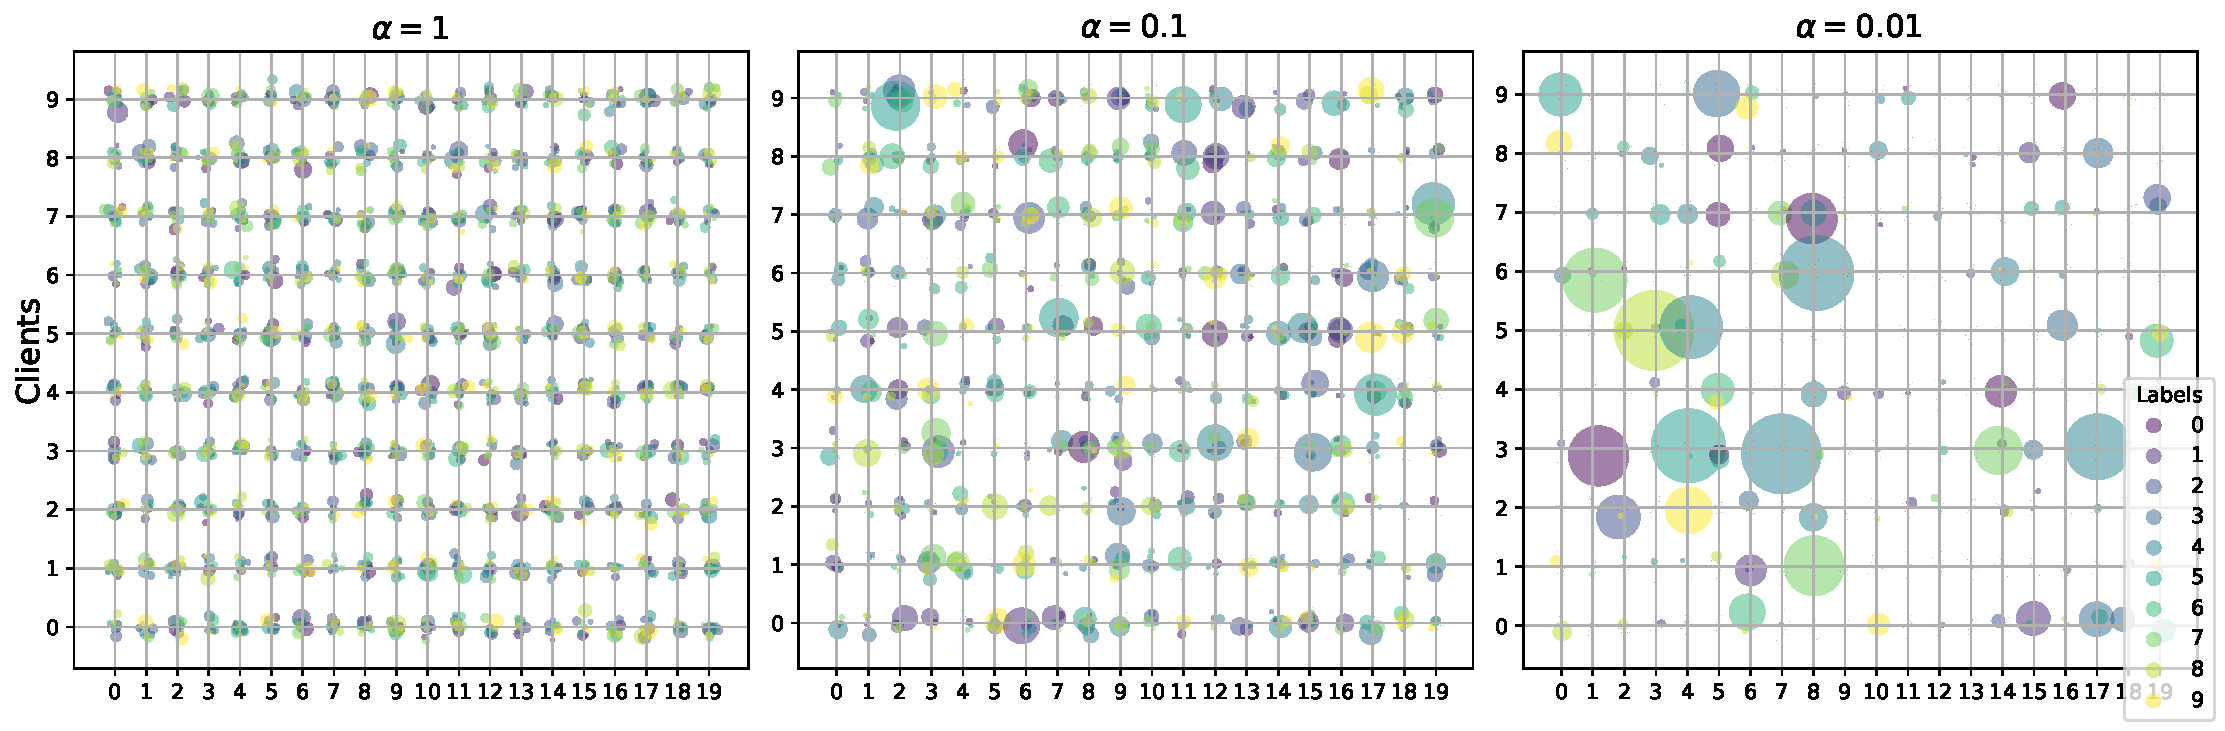
\includegraphics[width=0.8\linewidth]{noniid.pdf}}
%   % %\vspace{-2mm}
%   \subfigure[Visualization of its impact on performance]{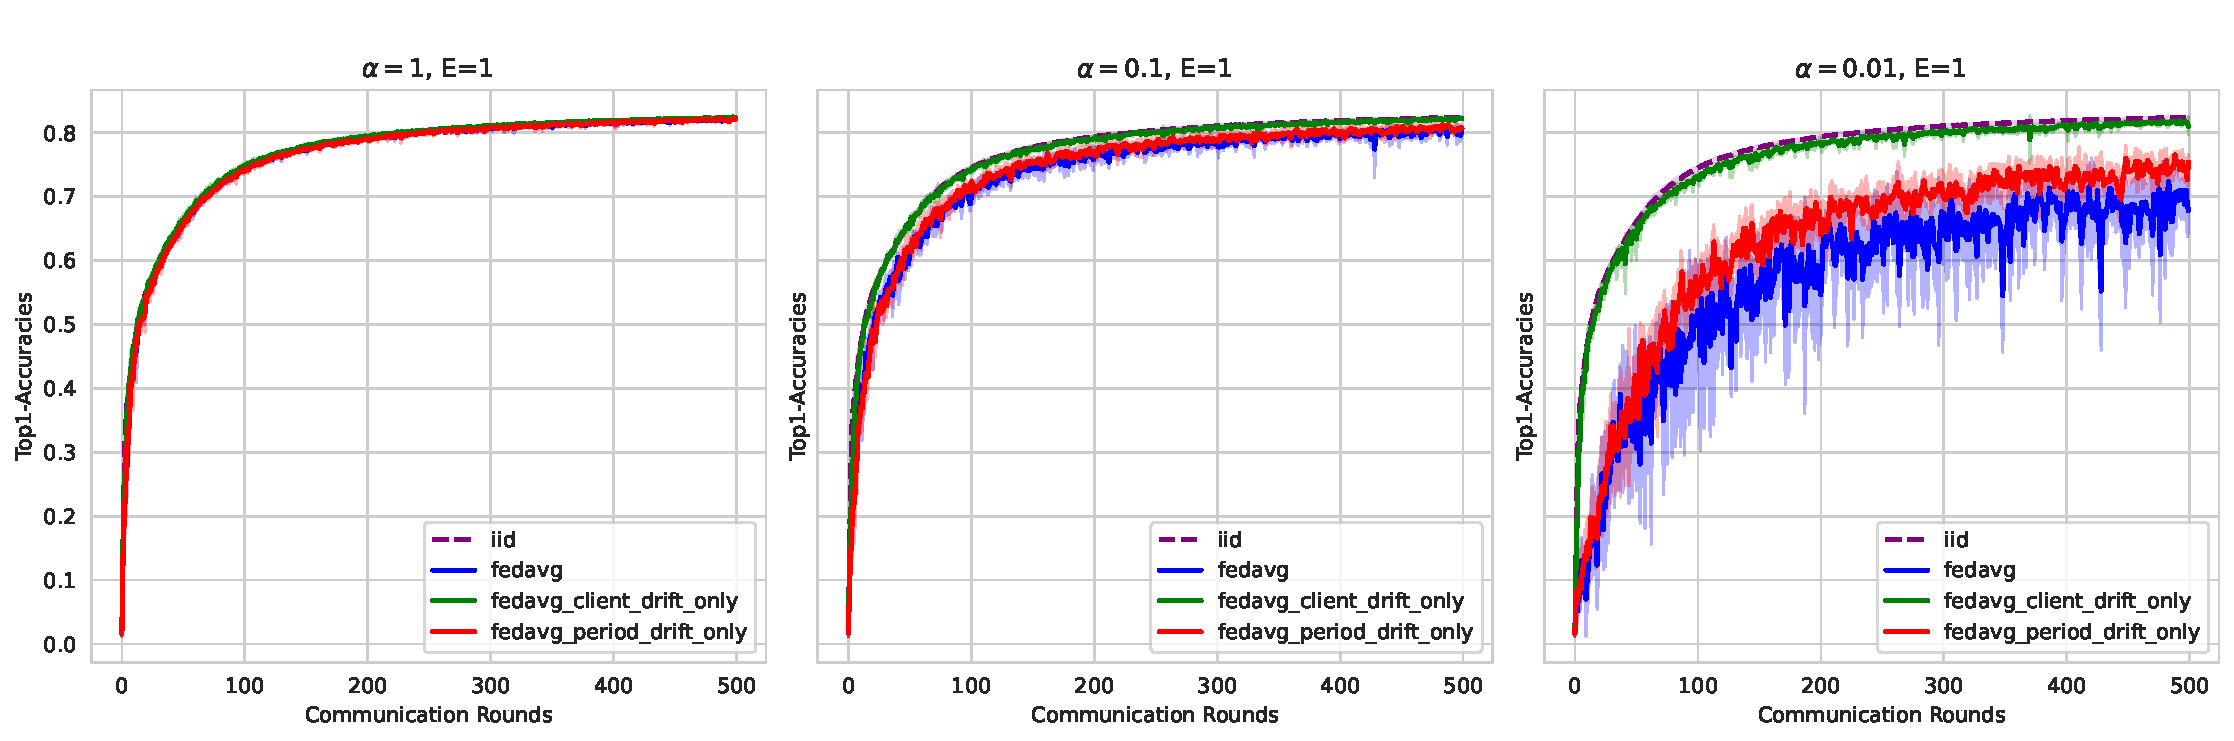
\includegraphics[width=0.8\linewidth]{seperate.pdf}}
%   %\vspace{-3mm}
%    \caption{\small \textbf{Visualization of period drift and its impact on performance.} 
%    % In each subfigure, a scatter plot is presented in which the x-axis represents 20 communication rounds, and the y-axis represents 10 randomly selected clients that vary between rounds. 
%    \textbf{(a) Visualization of period drift.} The color of the scatter points represents different classes, and the size denotes the number of samples of a given class on a particular client. When data is more non-iid (smaller $\alpha$), the heterogeneity of sampled data distributions becomes more pronounced both within a given communication round (\emph{client drift}) and between different communication rounds (\emph{period drift}). \textbf{(b) Visualization of its impact on performance.} It is revealed in cross-device FL when data is rather non-iid, period drift has a greater effect than client drift. Appendix for setting details.}
%    \label{fig:visualize}
%  \end{figure}
 
\begin{figure}[hp]
  \centering
  %\vspace{-3mm}
  \resizebox{1\linewidth}{!}{
{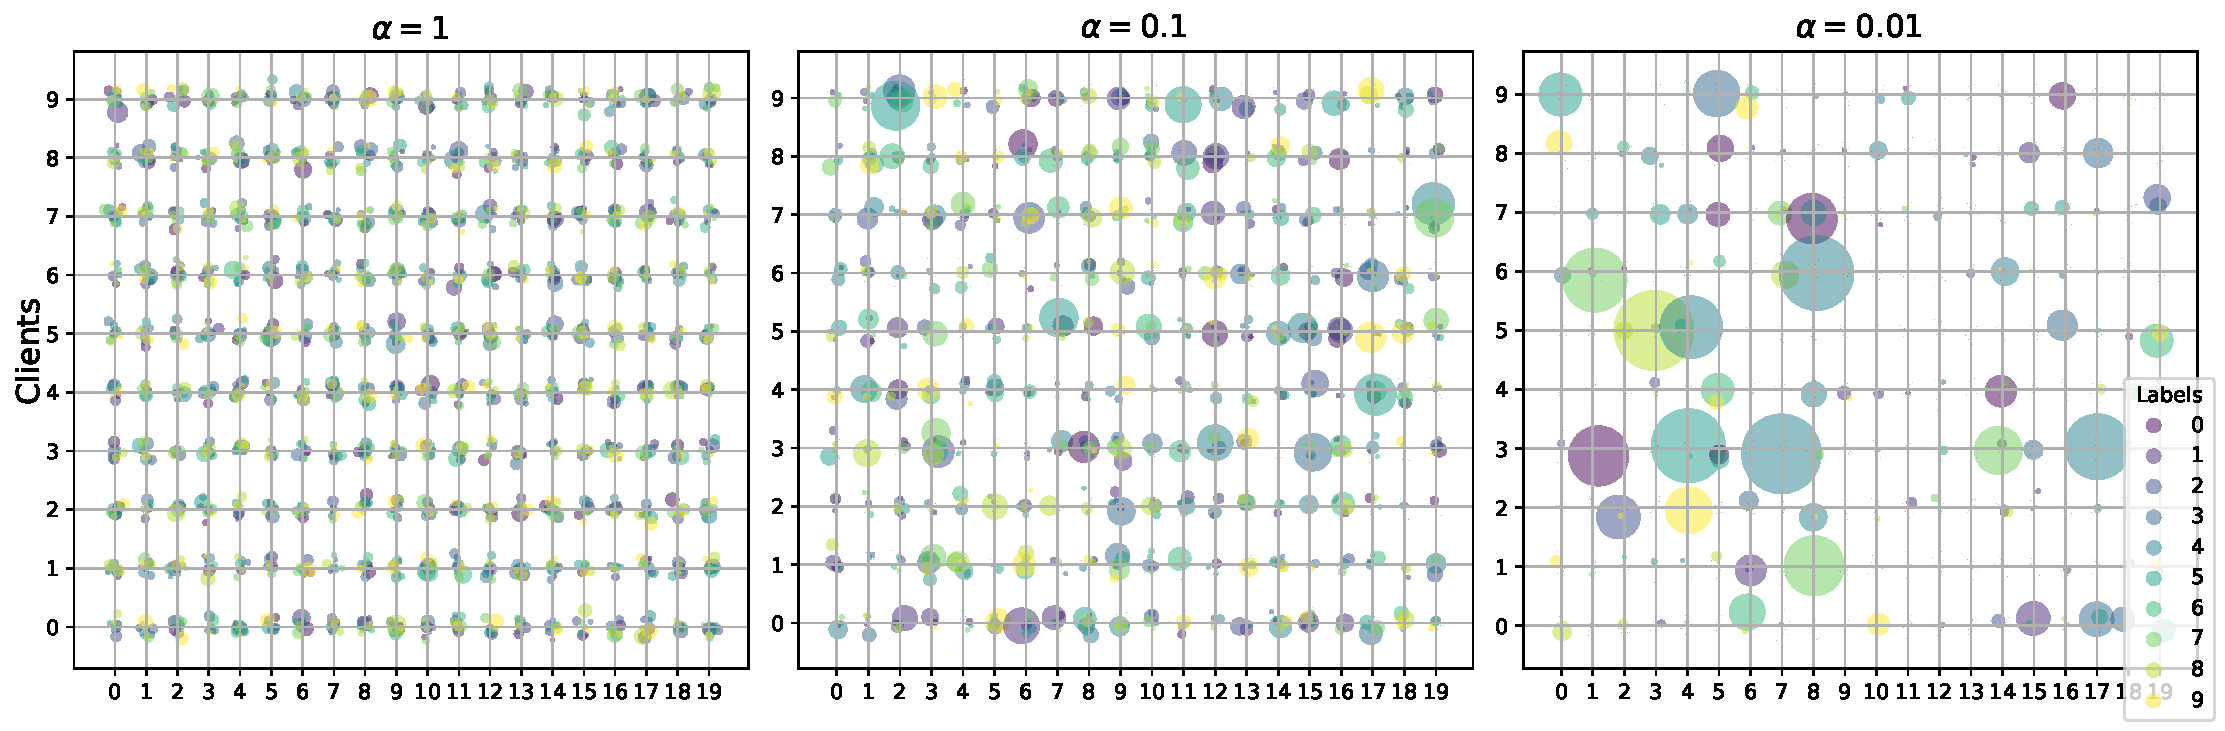
\includegraphics[width=0.95\linewidth]{noniid.pdf}}
 % %\vspace{-2mm}
{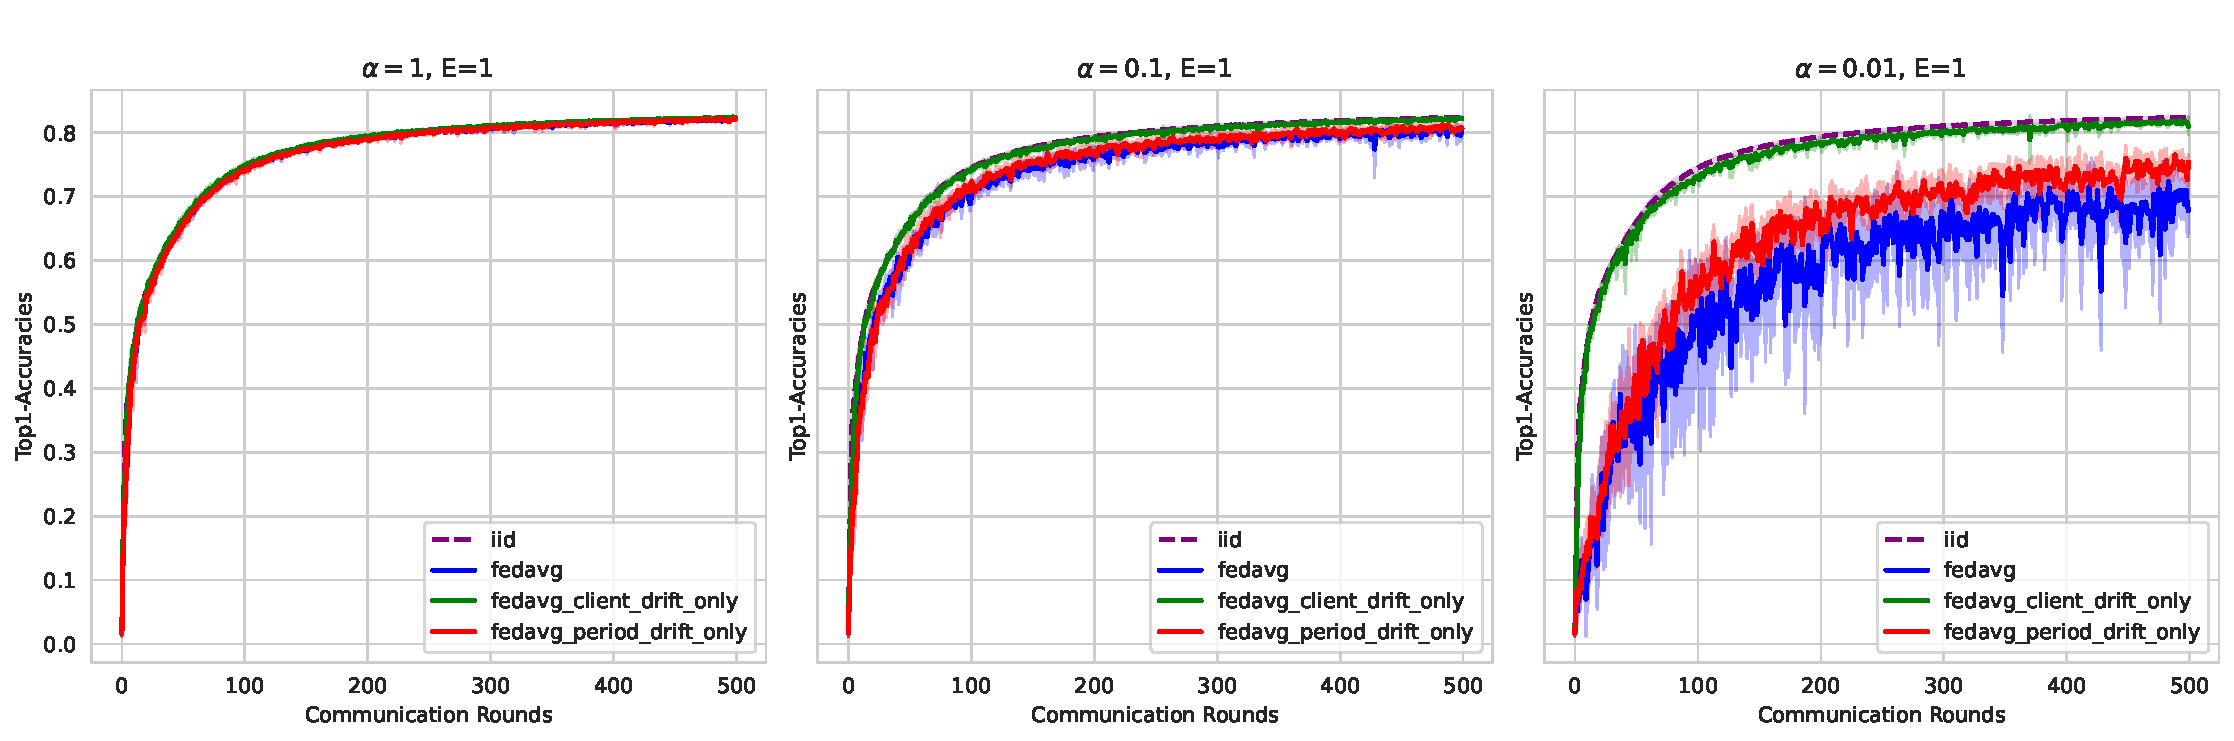
\includegraphics[width=1\linewidth]{seperate.pdf}}
 }
 \vspace{-3mm}

  \caption{
    \small \textbf{Visualization of period drift and its impact on performance} 
  % In each subfigure, a scatter plot is presented in which the x-axis represents 20 communication rounds, and the y-axis represents 10 randomly selected clients that vary between rounds. 
  \textbf{(a) Visualization of period drift} The color of the scatter points represents different classes, and the size denotes the number of samples of a given class on a particular client. 
  % When data is more non-iid (smaller $\alpha$), the heterogeneity of sampled data distributions becomes more pronounced both within a given communication round (\emph{client drift}) and between different communication rounds (\emph{period drift}). 
  \textbf{(b) Visualization of its impact on performance} It is revealed in cross-device FL when data is rather non-iid, period drift has a greater effect than client drift. Appendix \ref{sec:visualize} for setting details.}
  \label{fig:visualize}
  
  %\vspace{-5mm}
\end{figure}
\textbf{Visualizing the period drift and its impact.}
% In Figure \ref{fig:visualize}, we analyzed the phenomenon of non-iid data in cross-device FL environments using the FEMNIST dataset, focusing on period drift and client drift. Through simulating random client sampling, selecting 10 clients out of 3400 per round, 
Figure \ref{fig:visualize} (a) visualizes the data distributions of these sampled clients. Client drift arises due to the shift in label distribution among sampled clients \textbf{\textit{within a single round}}, while period drift results from the shift in the data distribution of participating clients \textbf{\textit{across different rounds}}. The scatter points' size and distribution grow more diverse both within and across communication rounds as the value of $\alpha$ decreases (indicating increasing non-iid). The implications of these drifts on the global model's convergence are presented in Figure \ref{fig:visualize} (b). Utilizing the vanilla \fedavg algorithm for illustration, we experimented with four settings: 1) \fedavg with iid data; 2) \fedavg experiencing only period drift; 3) \fedavg subject to only client drift; and 4) \fedavg impacted by both drifts (See appendix \ref{sec:visualize} for detailed settings). As heterogeneity intensifies, the effects of both drifts become evident. Specifically, in a highly non-iid environment ($\alpha=0.01$), \fedavg affected only by client drift yields results akin to the iid setting. In contrast, \fedavg influenced solely by period drift significantly disrupts the stability and convergence of the FL process. The combination of both drifts results in the poorest performance, underlining that in cross-device FL, period drift poses a more considerable challenge to model convergence than client drift. \looseness=-1
% \textbf{Visualizing the period drift and client drift.}
% In Figure \ref{fig:visualize}, we utilized the FEMNIST dataset to analyze the phenomenon of non-iid data, specifically period drift and client drift, in cross-device FL environments. We simulated random client sampling in cross-device FL, selecting 10 clients out of 3400 clients per round. We visualize the data distributions of the sampled 10 clients in Figure \ref{fig:visualize} (a). 
% Client drift is considered to be caused by the shift in label distribution among sampled clients \textbf{\textit{within a single round}}, while period drift is caused by the shift in the data distribution of participating clients \textbf{\textit{across different rounds}}. It illustrates that as the value of $\alpha$ decreases (more non-iid), the size and distribution of scatter points become more diverse both within the same communication round and between different rounds, indicating varying levels of client drift and period drift, respectively.

% % \begin{figure*}[!t]
% %   \centering
% %   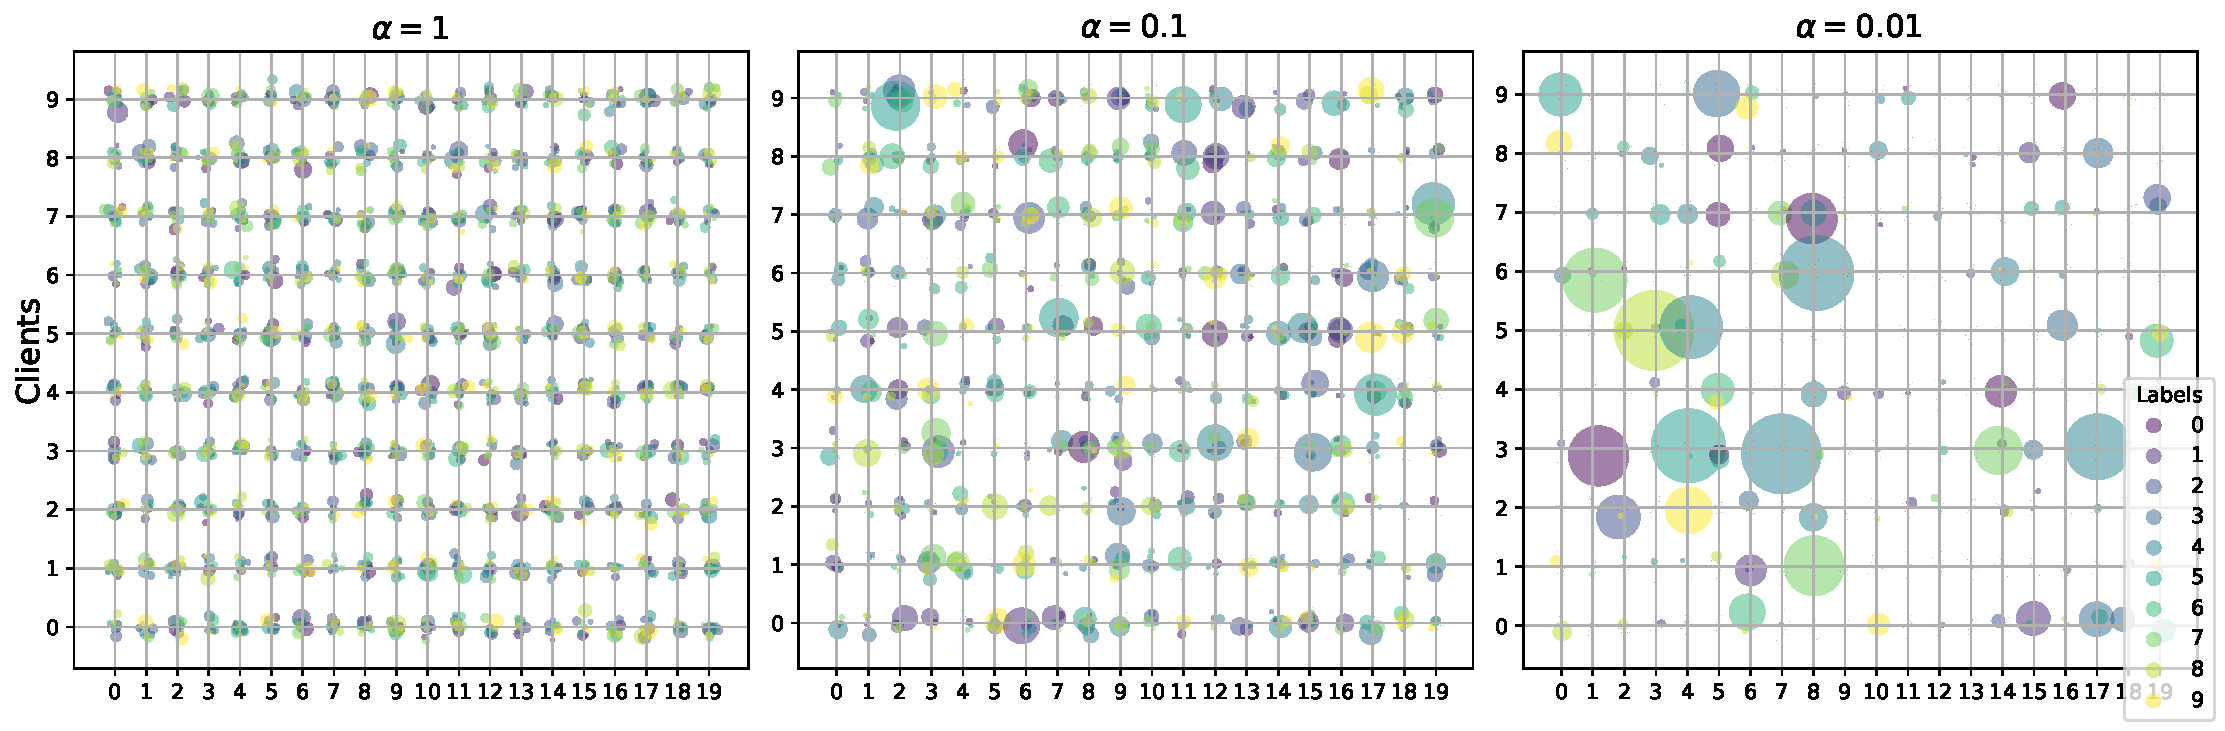
\includegraphics[width=\linewidth]{noniid.pdf}\label{fig:visualize}
% % %   \includegraphics[width=0.8\linewidth]{show_period.pdf}\label{show_period}
% %   \caption{\textbf{Visualize the period drift and client drift} In each subfigure, a scatter plot is presented in which the x-axis represents 20 communication rounds, and the y-axis represents 10 randomly selected clients that vary between rounds. The size of the scatter points reflects the number of samples of a given class label on a particular client, and the color of the scatter points represents different class labels. By decreasing the Dirichlet parameter $\alpha$ (which increases the level of non-iidness), the diversity of the size and distribution of scatter points becomes more pronounced both within a given communication round and between different communication rounds, indicating an increase in both client drift and period drift.}
% % \end{figure*}

% % put it in appendix: \fedavg with iid data, where training data is randomly partitioned among all clients, resulting in no period or client drift; \fedavg with iid data for each client, where non-iid data is partitioned initially, but training data is randomly reshuffled and distributed evenly among clients, resulting in period drift but no client drift; 3) \fedavg with iid data for each period, where data is initially partitioned iid, but training data is re-partitioned in non-iid setting, resulting in client drift but no period drift; 4) \fedavg with non-iid data, where data is partitioned in non-iid setting, resulting in both period and client drift, shown in Figure \ref{fig:seperate}.

% \textbf{The impact of period drift and client drift.} 
% We also showcase the impact of period drift and client drift on the global model's convergence in Figure \ref{fig:visualize} (b). 
% The vanilla \fedavg algorithm is adopted for simple illustration, and we conduct four different settings: 1) \fedavg with iid data with no period or client drift; 2) \fedavg with only period drift; 3) \fedavg with only client drift; 4) \fedavg with both period and client drift\footnote{Please refer to the appendix \ref{sec:visualize} for the setting details.}. As the level of heterogeneity increases, the impact of period drift and client drift becomes more prominent. For the extremely non-iid setting ($\alpha=0.01$), When using \fedavg with only client drift, the results are similar to that of the iid setting, but when using \fedavg with only period drift, it has a more significant impact on the stability and convergence of the FL process; further, if \fedavg is with both client and period drift, the performance is the worst. The results from the four experimental settings showed that in cross-device FL, period drift had a more substantial effect on the convergence of the model than client drift.
% \begin{table}[t]
%     \footnotesize
%     \centering
%       % %\vspace{-0.5cm}
%     \caption{\small\textbf{Results on FEMNIST and CIFAR-100.} The best method is highlighted in \textbf{bold} fonts.}
%     % %\vspace{-1em}
%     \resizebox{\linewidth}{!}{
%     \begin{tabular}{l|cccc|ccc}
%     \toprule
%     Dataset&\multicolumn{4}{c}{FEMNIST}&\multicolumn{3}{c}{CIFAR-100}\\
%     \cmidrule(lr){1-5}
%     \cmidrule(lr){6-8}
%     % \midrule 
%     Methods/NonIID &natural &$\alpha=1$ &$\alpha=0.1$ &$\alpha=0.01$&$\alpha=1$ &$\alpha=0.1$ &$\alpha=0.01$\\
%     \midrule
%     \fedavg & 82.37 $\pm$ 0.10 &83.60 $\pm$ 0.04 & 82.02 $\pm$ 0.16 &73.23 $\pm$ 1.26 &47.04 $\pm$ 0.21 &43.93 $\pm$ 0.36 & 30.11 $\pm$ 0.53 \\
%     \fedavgm & 82.53 $\pm$ 0.15 &83.68 $\pm$ 0.04 & 82.30 $\pm$ 0.13 &74.96 $\pm$ 1.25 & 48.22 $\pm$ 0.19 & 44.74 $\pm$ 0.40 &31.59 $\pm$ 0.98 \\
%     \fedprox & 82.34 $\pm$ 0.10 &83.58 $\pm$ 0.04 &82.04 $\pm$ 0.15 &74.16 $\pm$ 0.98 &46.86 $\pm$ 0.38 &43.74 $\pm$ 0.27 &30.10 $\pm$ 0.55 \\
%     \scaffold & 5.13 $\pm$ 0.00 &83.06 $\pm$ 0.08 &48.91 $\pm$ 35.75 &5.13 $\pm$ 0.00 &47.26 $\pm$ 1.49 &36.36 $\pm$ 4.98 &1.00 $\pm$ 0.00 \\
%     \fedopt & 5.13 $\pm$ 0.00 &82.06 $\pm$ 0.08 & 78.27 $\pm$ 0.38 &16.66 $\pm$ 23.06 &47.26 $\pm$ 1.49 &\textbf{47.71 $\pm$ 1.18}&32.17 $\pm$ 1.38 \\
%     \midrule
%     \textbf{\fedeve}&\textbf{82.68 $\pm$ 0.08} &\textbf{83.80 $\pm$ 0.04} &\textbf{82.63 $\pm$ 0.11} &\textbf{75.03 $\pm$ 1.13} &\textbf{48.38 $\pm$ 0.24} &45.68 $\pm$ 0.16 &\textbf{32.68 $\pm$ 0.62} \\
%     \bottomrule
%     \end{tabular}
%     }
%     \label{tab:femnist_cifar100}
%     % %\vspace{-0.2cm}
% \end{table}


\begin{table*}[t!]
    \centering
    \caption{\small\textbf{Results on FEMNIST with different $\alpha$ and $E$.} The best method is highlighted in \textbf{bold} fonts.}
    \label{tab:femnist}
    \resizebox{\linewidth}{!}{
    \begin{tabular}{l*{12}{c}}
        \toprule
        \multirow{2}{*}{Method} & \multicolumn{3}{c}{Natural} & \multicolumn{3}{c}{$\alpha=1$} & \multicolumn{3}{c}{$\alpha=0.1$} & \multicolumn{3}{c}{$\alpha=0.01$} \\
        \cmidrule(lr){2-4} \cmidrule(lr){5-7} \cmidrule(lr){8-10} \cmidrule(lr){11-13}
        & $E=1$ & $E=3$ & $E=5$ & $E=1$ & $E=3$ & $E=5$ & $E=1$ & $E=3$ & $E=5$ & $E=1$ & $E=3$ & $E=5$ \\
        \midrule
        % \rowcolor{Gray} 
        \fedavg & 82.46 $\pm$ 0.18 & 81.95 $\pm$ 0.26 & 66.38 $\pm$ 30.63 & 83.64 $\pm$ 0.11 & 83.57 $\pm$ 0.12 & 83.38 $\pm$ 0.09 & 82.12 $\pm$ 0.23 & 81.91 $\pm$ 0.23 & 81.70 $\pm$ 0.26 & 74.51 $\pm$ 1.36 & 73.43 $\pm$ 1.73 & 72.67 $\pm$ 1.39 \\
        \fedavgm & 82.55 $\pm$ 0.43 & 81.99 $\pm$ 0.42 & 50.97 $\pm$ 37.43 & 83.67 $\pm$ 0.10 & 83.79 $\pm$ 0.11 & 83.65 $\pm$ 0.08 & 82.36 $\pm$ 0.49 & 82.23 $\pm$ 0.26 & 82.16 $\pm$ 0.34 & 75.18 $\pm$ 2.34 & 74.20 $\pm$ 2.81 & 73.79 $\pm$ 3.13 \\
        % \rowcolor{Gray} 
        \fedprox & 82.43 $\pm$ 0.17 & 81.90 $\pm$ 0.27 & 51.07 $\pm$ 37.51 & 83.62 $\pm$ 0.11 & 83.52 $\pm$ 0.14 & 67.65 $\pm$ 31.26 & 82.17 $\pm$ 0.27 & 82.12 $\pm$ 0.19 & 81.94 $\pm$ 0.30 & 75.07 $\pm$ 1.19 & 74.38 $\pm$ 1.46 & 60.22 $\pm$ 27.56 \\
        \scaffold & 81.66 $\pm$ 0.28 & 81.08 $\pm$ 0.36 & 80.76 $\pm$ 0.30 & 83.18 $\pm$ 0.14 & 82.75 $\pm$ 0.16 & 82.46 $\pm$ 0.16 & 79.82 $\pm$ 0.42 & 79.00 $\pm$ 0.65 & 78.44 $\pm$ 0.70 & 5.13 $\pm$ 0.00 & 5.13 $\pm$ 0.00 & 5.13 $\pm$ 0.00 \\
        % \rowcolor{Gray}
        \fedopt & 5.13 $\pm$ 0.00 & 5.13 $\pm$ 0.00 & 5.13 $\pm$ 0.00 & 81.86 $\pm$ 0.38 & 35.90 $\pm$ 37.69 & 35.66 $\pm$ 37.39 & 78.13 $\pm$ 0.39 & 5.13 $\pm$ 0.00 & 5.13 $\pm$ 0.00 & 5.13 $\pm$ 0.00 & 5.13 $\pm$ 0.00 & 5.13 $\pm$ 0.00 \\
        \rowcolor{Gray}
        \fedeve & \textbf{82.66 $\pm$ 0.19} & \textbf{82.20 $\pm$ 0.20} & \textbf{81.93 $\pm$ 0.16} & \textbf{83.81 $\pm$ 0.09} & \textbf{83.88 $\pm$ 0.08} & \textbf{83.72 $\pm$ 0.05} & \textbf{82.69 $\pm$ 0.31} & \textbf{82.66 $\pm$ 0.18} & \textbf{82.52 $\pm$ 0.19} & \textbf{75.99 $\pm$ 1.61} & \textbf{75.00 $\pm$ 2.24} & \textbf{74.56 $\pm$ 2.05} \\
        \bottomrule
    \end{tabular}}
    %\vspace{-5mm}
\end{table*}


\textbf{The performance of \fedeve.}
We evaluate our algorithm on real-world datasets and compare it with the relevant state-of-the-art methods in Tables \ref{tab:femnist_cifar100} and \ref{tab:ml-1m}. We conducted simulations on three datasets: FEMNIST, CIFAR-100, and MovieLens. The FEMNIST and Movielens datasets have a naturally-arising client partitioning setting in real-world FL scenarios, making them highly representative. For FEMNIST and CIFAR-100 datasets, each of the datasets includes three non-iid settings, established through the Dirichlet distribution partition method \citep{hsu2019measuring}. \textit{Generally, the results show that our proposed algorithm, \fedeve, consistently outperforms the baselines, and the performance gains are more dominant in more non-iid settings ($\alpha=0.01$).} We also conduct experiments with different local epochs ($E$), please refer to the Figure \ref{fig:diff} for the setting details. Also, our \fedeve has more leading advantages in RS experiments, indicating its large potential in real-world industrial applications. 
% For the baselines, we find \fedavgm and \fedopt perform the best, revealing that the server-side momentum and adaptive methods are beneficial to cross-device FL with partial sampling, which is consistent with our insights on the period drift.
Our method can better utilize the server-side adaptation through the Bayesian filter's predict-observer framework. Besides, it is important to note that our method does not introduce other hyperparameters while these baselines have multiple hyperparameters to tune, which means that our \fedeve is more flexible and advantageous in real-world practices. 
% %\vspace{-10mm}

\textbf{Performace of \fedeve on FEMNIST with different local epochs.}\label{sec:different local epochs}
Table~\ref{tab:femnist} showcases the results on the FEMNIST dataset across various methods, specifically: \fedavg, \fedavgm, \fedprox, \scaffold, \fedopt, and \fedeve, with different settings of parameters $\alpha$ and $E$. \fedeve method stands out consistently as the superior approach across all configurations. This consistent performance signifies that \fedeve is a potent and reliable method for the FEMNIST dataset across the tested configurations.
The performance drop of SCAFFOLD in specific experiments may be attributed to two primary reasons:
Staleness of control variate: SCAFFOLD mandates that each client maintain a control variant. However, given the large number of clients and the fact that only a limited subset is chosen for training during each communication round, most control variants remain outdated. As a result, they fail to effectively correct the bias in local updates. This point was also reported in FedOpt~\citep{reddi2020adaptive}.
Excessiveness of correction: Upon detailed inspection of our experiments, we discerned that the training of SCAFFOLD tends to fail when there exists a client with more substantial data than others. This stems from the fact that the fixed batch size and training epoch will result in more local updates in the clients with more data, but it will be corrected by the same control variant in SCAFFOLD. Excessive corrections drive the model further from the optimal point, resulting in the divergence of the model.
We reckon that the poor performances of FedOpt in some settings primarily result from period drift. Period drift impedes FedOpt's adaptivity across rounds. FedOpt tailors the learning rates of individual weights by accumulating past gradients' squares.
However, with the ever-shifting optimization objectives in each communication round (period drift), these rate adjustments become misaligned for subsequent updates, thereby skewing model training.
It is validated in the experiments that FedOpt fails on FEMNIST with natural and 
 heterogeneity, where period drift is more dominant (more client number, more non-i.i.d. data).

 \begin{figure}[t]
  \centering
 \includegraphics[width=0.8\linewidth]{training_accuracy_across_settings_with_correct_zoom_and_fedeve.pdf}\label{fig:diff}
%  %\vspace{-6mm}
  \caption{\small \textbf{Accuracies with different $\alpha$ and $E$}}
  % %\vspace{-5mm}
\end{figure}

% \textbf{Analysis of Kalman Gain in \fedeve.} We conducted an in-depth analysis of the Kalman Gain $K$ 
% \begin{wrapfigure}{r}{0.5\textwidth}
%   \centering
%   \label{fig:kalman_gain}
%   \includegraphics[width=\linewidth]{fedeve_Kalman.pdf}
%   \caption{\small\textbf{Boxplots for Kalman Factors}}
% \end{wrapfigure}
% % \begin{figure}[ht]
% %   \centering
% %   % %\vspace{-4mm}
% %   \includegraphics[width=\linewidth]{fedeve_Kalman.pdf}\label{fig:kalman_gain}
% %   %\vspace{-6mm}
% %   \caption{\small\textbf{Boxplots for Kalman Factors}}
% %   %\vspace{-5mm}
% %   \end{figure}
%  of FedEve under various experimental settings, incorporating four levels of data heterogeneity and various local epochs, as shown in Figure 4. We observed that as data heterogeneity increases (i.e., as the value of $\alpha$ decreases), the Kalman Gain $K$ progressively enlarges. With the rise of data heterogeneity, the period drift starts to play a more dominant role. In this context, the primary role of Kalman Gain $K$ is to adjust the weights between global and local updates, as depicted by Equation (\ref{step:pre_s}) and (\ref{step:G_kal}). Further, according to Equation (\ref{step:M}), the model update tends to trust local updates more, stabilizing the optimization process. For varied counts of local updates, the relative change in Kalman Gain $K$ is marginal. This is primarily because, in cross-device FL, the client drift is not a pivotal or dominant factor, which aligns with our prior analysis in Figure \ref{fig:visualize}.



%     \begin{figure}[t]
%     \centering
%     \includegraphics[width=0.6\linewidth]{fedeve_Kalman.pdf}
%     \caption{\small \textbf{Boxplots for Kalman Factors}}
% \end{figure}
% \begin{itemize}
%    \item \fedavg with iid data, where training data is randomly partitioned among all clients, resulting in no period or client drift.
%    \item \fedavg with iid data for each client, where non-iid data is partitioned initially, but training data is randomly reshuffled and distributed evenly among clients, resulting in period drift but no client drift.
%    \item \fedavg with iid data for each period, where data is initially partitioned iid, but training data is re-partitioned in non-iid setting, resulting in client drift but no period drift.
%    \item \fedavg with non-iid data, where data is partitioned in non-iid setting, resulting in both period and client drift.
% \end{itemize}


% \begin{itemize}
%    \item \fedavg is applied to iid data, where the training data is randomly partitioned among all clients. As a result, there is no period drift or client drift observed in this scenario. This setup serves as a control group for comparison with the other experimental settings in which period drift and/or client drift are present.
%    \item \fedavg algorithm is applied to iid data for each client, where non-iid data is initially partitioned. However, the training data is randomly reshuffled and distributed evenly among clients. As a result, period drift is present but no client drift is observed. In other words, the data distribution among clients change over time, but the distribution of data remains the same for each individual client. This setting allows for the examination of the effect of period drift on the convergence of the \fedavg algorithm in cross-device federated learning (FL) separately from the effect of client drift.
%    \item \fedavg algorithm is applied to iid data for each period, where data is initially partitioned iid. However, the training data is re-partitioned in a non-iid setting, resulting in client drift but no period drift. In other words, the distribution of data remains the same over time for each individual client, but it becomes different across clients. This setting allows for the examination of the effect of client drift on the convergence of the \fedavg algorithm in cross-device federated learning (FL) separately from the effect of period drift. This setting is useful to understand how the different data distribution among clients affect the convergence.
%    \item \fedavg algorithm is applied to non-iid data, where data is partitioned in a non-iid setting, resulting in both period and client drift. This means that the distribution of data changes over time for each individual client, and it also becomes different across clients. This setting allows for the examination of the combined effect of period drift and client drift on the convergence of the \fedavg algorithm in cross-device federated learning (FL). This scenario represents a more realistic setup, where data is not always iid and it's not evenly distributed among clients, this setting can provide insights on how the algorithm behaves in such scenarios and how to improve the convergence in non-iid data distribution.
% \end{itemize}
% The above statement highlights that as the degree of non-iidness in the data increases, the complexity of federated learning (FL) training also increases. Furthermore, it is noted that period drift has a more significant impact on the stability and convergence of the FL process than client drift. The statement also suggests that through comparisons of the results obtained from the four experimental settings, it has been determined that in cross-device FL, period drift has a greater effect on convergence than client drift. This makes period drift a particularly challenging aspect of the FL process to overcome. This statement highlights the importance of understanding and mitigating period drift in cross-device FL to improve the stability and convergence of the training process.



%  \begin{figure*}[!t]
%    \centering
%    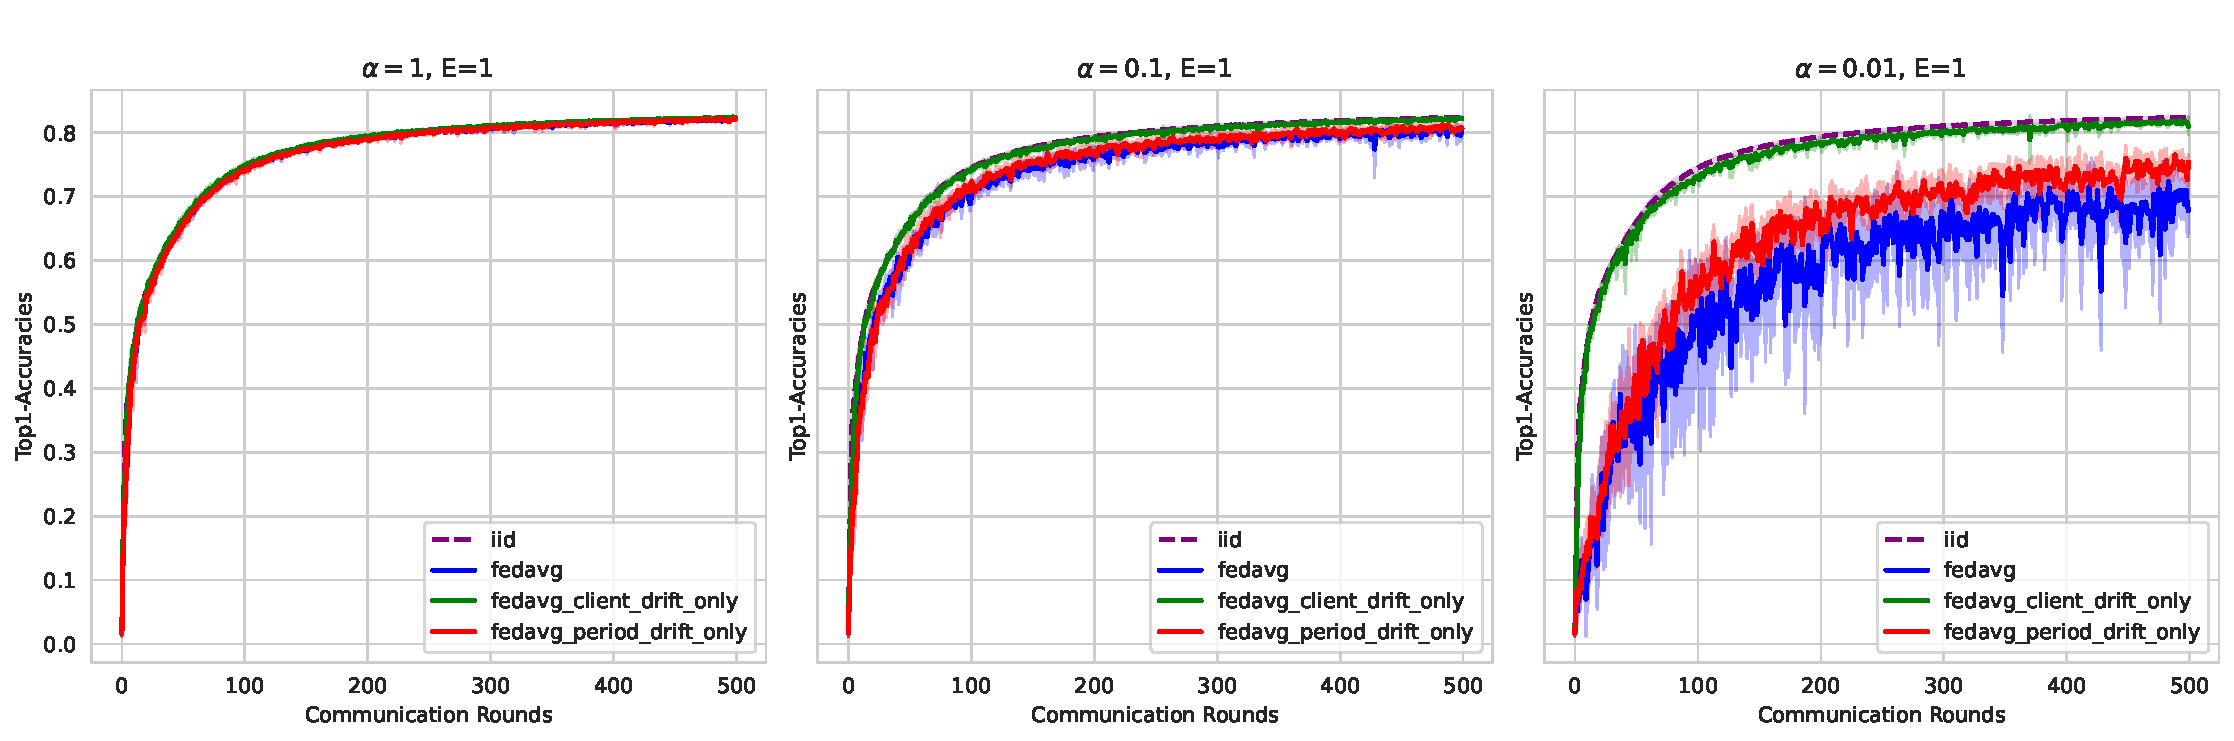
\includegraphics[width=\linewidth]{seperate.pdf}\label{fig:seperate}
%    \caption{\textbf{Visualize the period drift and client drift} In each subfigure, a scatter plot is presented in which the x-axis represents 20 communication rounds, and the y-axis represents 10 randomly selected clients that vary between rounds. The size of the scatter points reflects the number of samples of a given class label on a particular client, and the color of the scatter points represents different class labels. By decreasing the Dirichlet parameter $\alpha$ (which increases the level of non-iidness), the diversity of the size and distribution of scatter points becomes more pronounced both within a given communication round and between different communication rounds, indicating an increase in both client drift and period drift.}
%  \end{figure*}


% \begin{table}[!ht]
% \centering
% \caption{\textbf{The performance on FEMNIST}}\label{table:femnist}
% \begin{tabular}{lcccc}
% \toprule
% ~ & Natural & $\alpha=1$ & $\alpha=0.1$& $\alpha=0.01$\\ 
% \midrule
% \fedavg & $0.8243$ & $0.8353$ & $0.8207$ & $0.7332$\\
% \fedavgm & $0.8254$ & $0.8366$ & $0.8221$ & $0.7531$\\
% \fedprox & $0.8241$ & $0.835$ & $0.8209$ & $0.744$\\
% \fedopt & $0.0513$ & $0.8206$ & $0.7839$ & $0.5905$\\
% \fedeve & $\textbf{0.8266}$ & $\textbf{0.8371}$ & $\textbf{0.8257}$ & $\textbf{0.7554}$\\
% \bottomrule
% \end{tabular}
% \end{table}
% % %\vspace{-10mm}

% % \begin{table}[!ht]
% % \centering
% % \caption{\textbf{The performance on CIFAR10}}
% % \begin{tabular}{lccc}
% % \toprule
% % ~ & $\alpha=1$ & $\alpha=0.1$& $\alpha=0.01$\\ 
% % \midrule
% % 'fedavg' & $0.7447$ & $0.6897$ & $0.1$\\
% % 'fedavgm' & $0.5397$ & $0.4937$ & $0.1$\\
% % 'fedprox' & $0.7479$ & $0.6864$ & $0.1$\\
% % 'fedopt' & $0.8004$ & $0.7242$ & $0.1$\\
% % 'fedeve' & $0.728$ & $0.6929$ & $0.1$\\
% % \bottomrule
% % \end{tabular}
% % \end{table}
% % %\vspace{-10mm}
% \begin{table}[!ht]
% \centering
% \caption{\textbf{The performance on }}\label{table:cifar100}
% % \setlength{\tabcolsep}{4mm}
% {
% \begin{tabular}{lccc}
% \toprule
% ~ & $\alpha=1$ & $\alpha=0.1$& $\alpha=0.01$\\ 
% \midrule
% \fedavg & $\textbf{0.4680}$ & $\textbf{0.4399}$ & $0.291$\\
% \fedavgm & $0.2431$ & $0.2103$ & $0.139$\\
% \fedprox & $0.4661$ & $0.4386$ & $0.2913$\\
% \fedopt & $0.4539$ & $0.3479$ & $0.1124$\\
% \fedeve & $0.4301$ & $0.4368$ & $\textbf{0.2927}$\\
% \bottomrule
% \end{tabular}}
% \end{table}
% \begin{table}[!ht]
%    \centering
%    \caption{\textbf{The performance on MovieLens 1M}}\label{table:ml-1m}
%    \resizebox{\linewidth}{!}
%    {
%    \begin{tabular}{lccccc}
%    \toprule
%        ~ & \textbf{Auc} & \textbf{HR@5} & \textbf{HR@10}& \textbf{NDCG@5} & \textbf{NDCG@10} \\ 
%    \midrule
%    \fedavg & $0.7979$ & $\textbf{0.2887}$ & $0.4389$ & $0.1883$ & $0.2365$\\
%    \fedavgm & $0.7623$ & $0.2752$ & $0.4311$ & $0.1704$ & $0.2210$\\
%    \fedprox & $0.7615$ & $0.2827$ & $0.431$ & $0.181$ & $0.2288$\\
%    \fedopt & $0.6570$ & $0.1582$ & $0.2773$ & $0.0960$ & $0.1344$\\
%    \fedeve & $\textbf{0.7986}$ & $0.2875$ & $\textbf{0.4399}$ & $\textbf{0.1928}$ & $\textbf{0.2417}$\\
%    % \feddf & $0.7053$ & $0.2553$ & $0.3623$ & $0.1701$ & $0.2046$ \\ 
%    % \fedmeta & $0.7651$ & $0.2930$ & $0.4429$ & $0.1919$ & $0.2404$ \\ 
%    % \fedpa & $0.7878$ & $0.3058$ & $0.4382$ & $0.2002$ & $0.2431$ \\
%    \bottomrule
%    \end{tabular}}
%  \end{table}